\documentclass{article}

\usepackage[spanish]{babel}
\usepackage{graphicx} % Required for the inclusion of images
\usepackage{amsmath} % Required for some math elements 
\usepackage{hyperref}
\usepackage{amsmath}
\usepackage{listings}
\usepackage{xcolor}
\usepackage{courier}
\usepackage[margin=1in]{geometry}
\usepackage{changepage}
\usepackage{titlesec}
\usepackage{wrapfig}
\usepackage[version=4]{mhchem}
\usepackage{multirow}
\usepackage{siunitx}
\usepackage{ragged2e}
\usepackage{adjustbox}
\usepackage{caption}

\definecolor{codegreen}{rgb}{0,0.6,0}
\definecolor{codegray}{rgb}{0.5,0.5,0.5}
\definecolor{codepurple}{rgb}{0.58,0,0.82}
\definecolor{backcolour}{rgb}{0.95,0.95,0.92}

\lstdefinestyle{mystyle}{
    backgroundcolor=\color{backcolour},   
    commentstyle=\color{codegreen},
    keywordstyle=\color{magenta},
    numberstyle=\tiny\color{codegray},
    stringstyle=\color{codepurple},
    basicstyle=\ttfamily\footnotesize,
    breakatwhitespace=false,         
    captionpos=b,                    
    keepspaces=true,                 
    numbers=left,                    
    numbersep=5pt,                  
    showspaces=false,                
    showstringspaces=false,
    showtabs=false,                  
    tabsize=2
}
\lstset{language=Python, 
        basicstyle=\ttfamily\small, 
        keywordstyle=\color{keywords},
        commentstyle=\color{comments},
        stringstyle=\color{red},
        showstringspaces=false,
        identifierstyle=\color{codepurple},
        keywords=[2]{pow},
        keywordstyle=[2]{\color{orange}},
}

\lstset{style=mystyle}
\setlength\parindent{0pt}
\renewcommand{\labelenumi}{\alph{enumi}.}

\title{\textbf{Análisis de circuitos \\ de corriente alterna}}

\author{Víctor Mira Ramírez}

\date{\today}

\begin{document}

\maketitle

\begin{center}
\begin{tabular}{l r}

Profesor: & Carlos Untiedt Lecuona\\
Lugar: & Universidad de Alicante
\end{tabular}
\end{center}

\vspace{2cm}
\tableofcontents

\vspace{2cm}
\begin{abstract}
\noindent En esta práctica de ordenador vamos a estudiar mediante el uso de programas en el lenguaje python, la dinámica de circuitos RLC con o sin generador. Para ello resolveremos diferentes ecuaciones diferenciales, regulando su dinámica mediante el uso de algoritmos. Representaremos los resultados de las magnitudes obtenidas utilizando gráficas en función del tiempo.\\ \\Analizaremos oscilaciones amortiguadas, tanto subamortiguadas como sobreamortiguadas, así como el caso con oscilaciones no amortiguadas.
\end{abstract}
    
\clearpage
    
\section{Circuito RLC en serie sin generador}
    El sistema que estudiaremos es el mostrado en la figura 1: Un condensador inicialmente cargado $Q$, una resistencia $R$, una bobina $L$ y un interruptor abierto $S$.

    \begin{figure}[h]
        \centering
        \begin{minipage}{.5\textwidth}
            \centering
            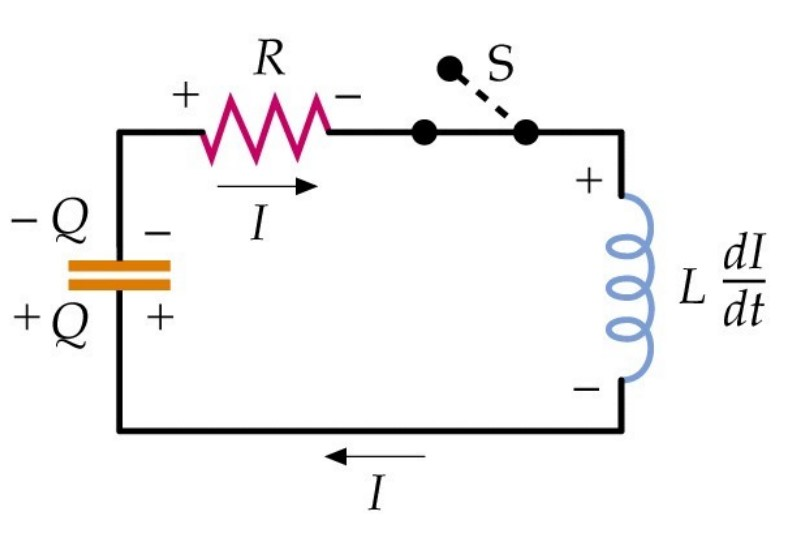
\includegraphics[width=.8\linewidth]{Fotos/RLCsin.jpg}
            \captionof{figure}{Circuito RLC}
        \end{minipage}%
        \begin{minipage}{.5\textwidth}
            \centering
            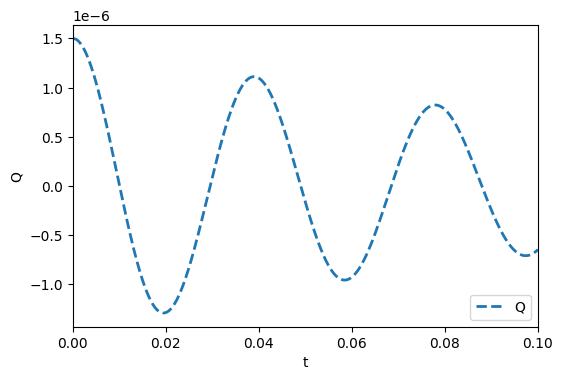
\includegraphics[width=.8\linewidth]{Fotos/SINq.png}
            \captionof{figure}{$Q$ respecto de $t$}
        \end{minipage}
    \end{figure}

    A tiempo cero se cierra el interruptor $S$ y se estudia como evoluciona el sistema. Este circuito se excita con la energía inicialmente almacenada en el condensador. Tal energía está representada por la tensión inicial del condensador $V_C$, o análogamente, con su carga inicial como podemos observar en la figura 2, cuyo decaimiento se explica por la resistencia efectiva o impedancia.\\
    
    Aplicando la regla de Kirchoff a la malla se obtiene:
    
    \[V_C(t)-V_R(t)-V_L(t)= 0\]
    
    donde $V_L = L \frac{dI}{dt}$ es el valor de la $fem$ de la bobina. \\
    
    Puede deducirse que la carga $Q$ del condensador satisface la siguiente ecuación diferencial homogénea ordinaria de segundo grado:
    
    \[L \frac{d^{2}Q}{dt^2}+R \frac{dQ}{dt}+ \frac{1}{C}Q=0\]
    
    Ahora, dividimos cada uno de los sumandos entre $L$ y obtenemos:
    
    \[ \frac{d^{2}Q}{dt^2}+\frac{R}{L} \frac{dQ}{dt}+ \frac{Q}{LC}=0\]
    
    Además, como la corriente que recorre el circuito es $ I= \frac{dQ}{dt}$, el cambio de variable que realizaremos para tener dos ecuaciones integrales de primer orden queda de la siguiente forma:
    
    \[
    \left.
    \begin{array}{rcl}
    \frac{dQ}{dt}=I\\
    \frac{dI}{dt}=-\frac{1}{L}(RI +\frac{Q}{C})\\
    \end{array}
    \right\}
    \]
    
    Ahora, ya tenemos dos ecuaciones diferenciales de primer orden, integrables con la función 'odeint' de la librería de python 'scipy'.\\
    
    La reactancia inductiva $X_L=wL $ y la reactancia capacitiva $X_C = \frac{1}{wC}$ desempeñan el papel de una resistencia efectiva en los circuitos puramente inductivos y capacitivos, respectivamente. En el circuito RLC en serie, la resistencia efectiva es la impedancia, $Z$, definida así:
    
    $$Z=\sqrt{R^2+(X_L-X_C)^2} $$
    \hfill
    
\clearpage
    
    \subsection{Oscilador no amortiguado}
    Cuando $R=0$, la ecuación diferencial de la carga queda así:

    \[\frac{dQ^2}{dt^2}=-\frac{1}{LC}Q\]
    
    Puede ponerse la ecuación anterior de la misma forma escribiendo $\omega^2$ en lugar de $1/LC$. Siendo la solución de la ecuación:
    \[Q=A \cos(\omega t - \delta)\]
    La corriente se halla derivando esta solución:
    \[I=\frac{dQ}{dt}=-\omega A \sin(\omega t - \delta)\]
    Escogiendo las condiciones iniciales que sean $Q=Q_0$ e $I=0$ en $t=0$, la constante de fase $\delta$ es nula y $A=Q_0$. Las soluciones quedan de la siguiente forma:
    
    \[Q=Q_0 \cos(\omega t)\ \ \ \ \ \ \ \ \ \ \ \ \ I=-\omega Q_0 \sin(\omega t)=-I_0 \sin{\omega t}\]
    
    Obtenemos para las energías eléctrica y magnética respectivamente, las siguientes ecuaciones:
    
    \[U_e=\frac{1}{2}QV=\frac{1}{2}CV^2=\frac{1}{2}\frac{Q^2}{C}\ \ \ \ \ \ \ \ \ \ \ \ \ \ \ \ \ \ \ U_m=\frac{1}{2}LI^2\]
    
    y para la frecuencia:
    
    \[f=\frac{1}{2\pi\sqrt{LC}}\]
    
    Con valores aleatorios obtenidos aleatoriamente representamos la intensidad y la carga frente al tiempo (Figuras 3 y 4), además de la energía magnética y eléctrica y su suma (Figuras 5 y 6). Obtenemos de las gráficas una frecuencia de oscilación de $25,700\ hz$ que coincide con el cálculo numérico, de $25,704\ hz$. En la figura 6 no obtenemos una línea completamente horizontal a causa del arrastre de errores en el código, aunque este error sea del orden de $10^{-8}\ J$
    
    \begin{figure}[h]
        \centering
        \begin{minipage}{.5\textwidth}
            \centering
            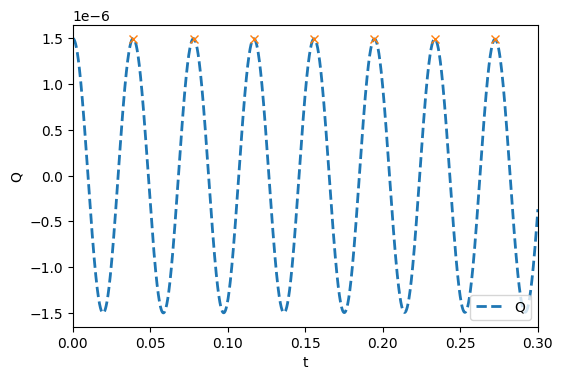
\includegraphics[width=.6\linewidth]{Fotos/SINno1.png}
            \captionof{figure}{$Q$ respecto de $t$}
        \end{minipage}%
        \begin{minipage}{.5\textwidth}
            \centering
            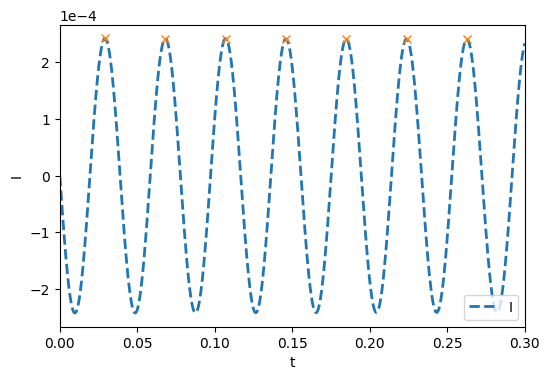
\includegraphics[width=.6\linewidth]{Fotos/SINno2.png}
            \captionof{figure}{$I$ respecto de $t$}
        \end{minipage}
    \end{figure}

    \begin{figure}[h]
        \centering
        \begin{minipage}{.5\textwidth}
            \centering
            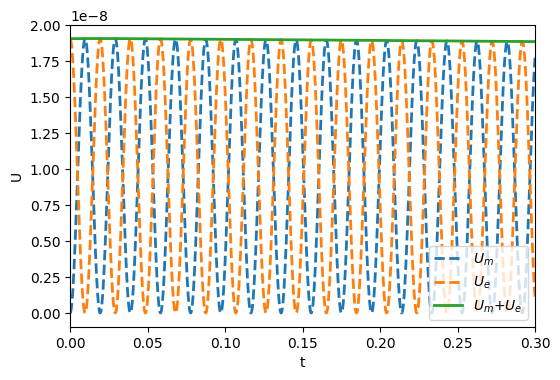
\includegraphics[width=.6\linewidth]{Fotos/SINno3.png}
            \captionof{figure}{Energías}
        \end{minipage}%
        \begin{minipage}{.5\textwidth}
            \centering
            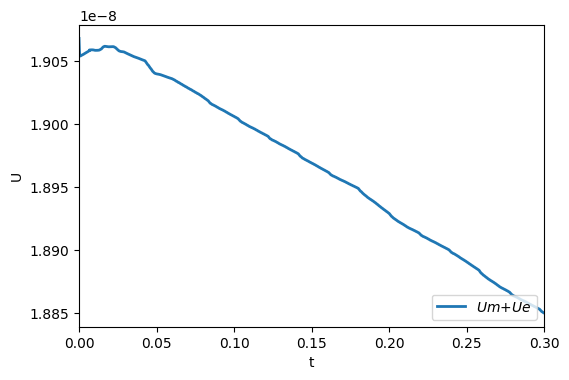
\includegraphics[width=.6\linewidth]{Fotos/SINno4.png}
            \captionof{figure}{Suma de ambas}
        \end{minipage}
    \end{figure}
    
\clearpage

    \subsection{Oscilador amortiguado}
        \vspace{0.4cm}
        \subsubsection{Oscilación subamortiguada}
        Con los mismos valores de $C$, $L$ y $Q_0$ usados en el apartado anterior, cambiaremos el valor de R poniendo un valor tal que $R^2 < \frac{4L}{C}$. Representaremos $Q=f(t)$, $I=f(t)$ y $U_m+U_e=f(t)$. de la misma forma. 
        
        \vspace{1.5cm}
        \begin{figure}[h]
            \centering
            \begin{minipage}{.5\textwidth}
                \centering
                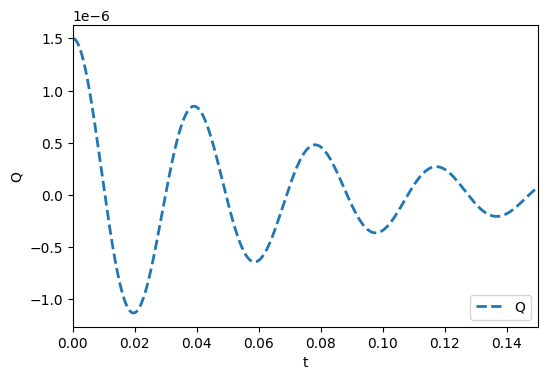
\includegraphics[width=1\linewidth]{Fotos/SINsub1.png}
                \captionof{figure}{$Q$ respecto de $t$}
            \end{minipage}%
            \begin{minipage}{.5\textwidth}
                \centering
                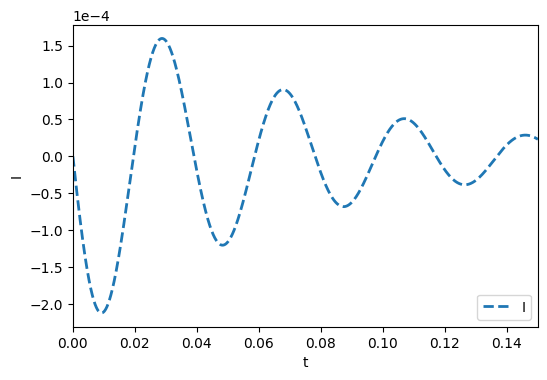
\includegraphics[width=1\linewidth]{Fotos/SINsub2.png}
                \captionof{figure}{$I$ respecto de $t$}
            \end{minipage}
        \end{figure}
        
        \vspace{0.4cm}
        \begin{figure}[h]
            \centering
            \begin{minipage}{.5\textwidth}
                \centering
                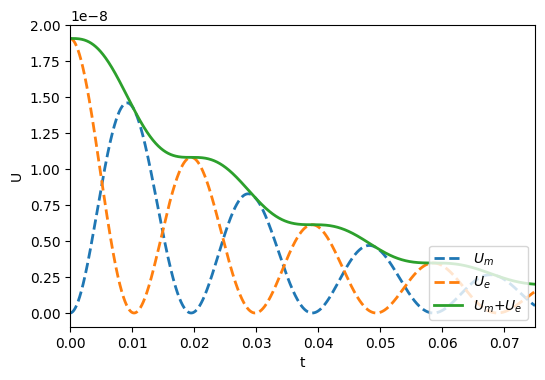
\includegraphics[width=1\linewidth]{Fotos/SINsub3.png}
                \captionof{figure}{Energías}
            \end{minipage}%
            \begin{minipage}{.5\textwidth}
                \centering
                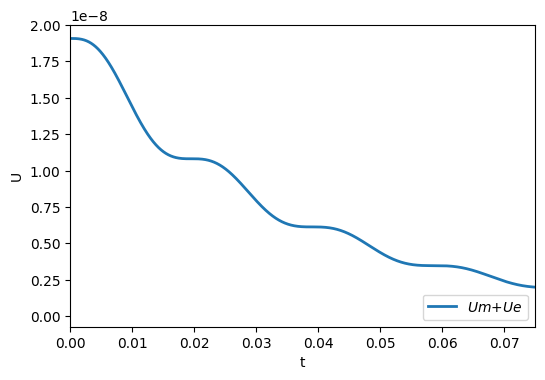
\includegraphics[width=1\linewidth]{Fotos/SINsub4.png}
                \captionof{figure}{Suma de ambas}
            \end{minipage}
        \end{figure}

\clearpage

        \subsubsection{Oscilación sobreamortiguada} 
        Con los mismos valores de $C$, $L$ y $Q_0$ usados en el apartado anterior, cambiaremos el valor de $R$ poniendo un valor tal que $R²>\frac{4L}{C}$. Representaremos $Q=f(t)$, $I=f(t)$ y $U_m+U_e=f(t)$ de la misma manera.
        
        \vspace{1.5cm}
        \begin{figure}[h]
            \centering
            \begin{minipage}{.5\textwidth}
                \centering
                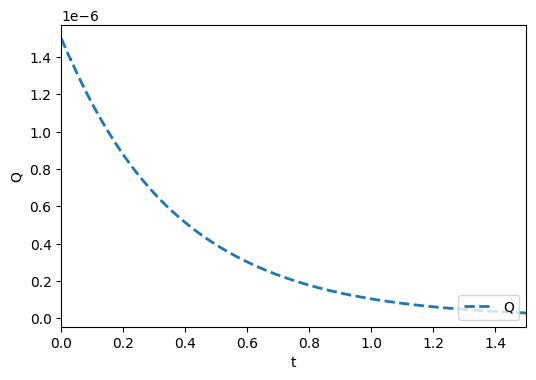
\includegraphics[width=1\linewidth]{Fotos/SINsob1.png}
                \captionof{figure}{$Q$ respecto de $t$}
            \end{minipage}%
            \begin{minipage}{.5\textwidth}
                \centering
                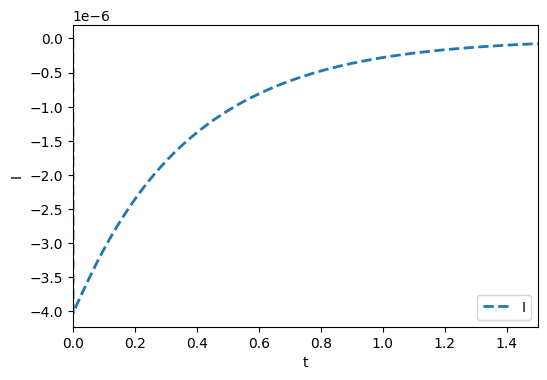
\includegraphics[width=1\linewidth]{Fotos/SINsob2.png}
                \captionof{figure}{$I$ respecto de $t$}
            \end{minipage}
        \end{figure}
    
        \vspace{0.4cm}
        \begin{figure}[h]
            \centering
            \begin{minipage}{.5\textwidth}
                \centering
                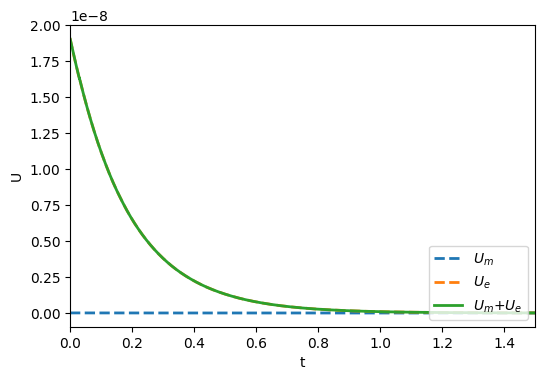
\includegraphics[width=1\linewidth]{Fotos/SINsob3.png}
                \captionof{figure}{Energías}
            \end{minipage}%
            \begin{minipage}{.5\textwidth}
                \centering
                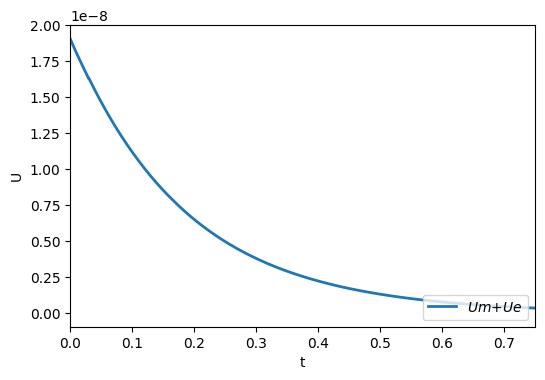
\includegraphics[width=1\linewidth]{Fotos/SINsob4.png}
                \captionof{figure}{Suma de ambas}
            \end{minipage}
        \end{figure}
        
\clearpage

    \subsection{Energía disipada por la resistencia}
        Conociendo $I(t)$ podemos calcular la energía total disipada en la resistencia como $$U_R=\int_0^\infty I^2(t)Rdt$$ 
    
        Graficamos $I(t)$ y calculamos $U_R$ eligiendo como intervalo superior un tiempo largo de manera que $I$ se haya hecho muy pequeña. Verificamos que $U_R$ es igual a la energía inicial del circuito que corresponde a la $U_e$ que tenía el condensador inicialmente. Presentamos gráficos tanto para casos subamortiguados como sobreamoritugados:\\ 
        
        $R = 10\ \Omega ,\ \ U_{r} = 1.904\cdot10^{-8}\ J$):
        
        \begin{figure}[h]
            \centering
            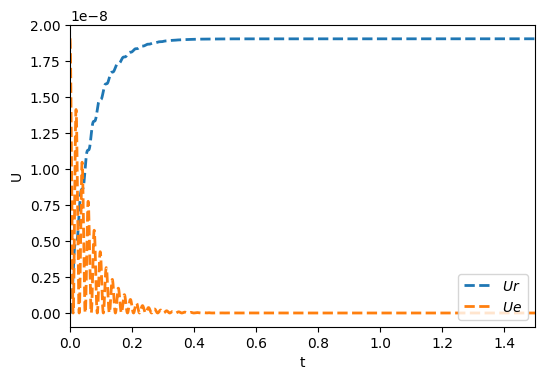
\includegraphics[width=.42\textwidth]{Fotos/SINen3.png}
            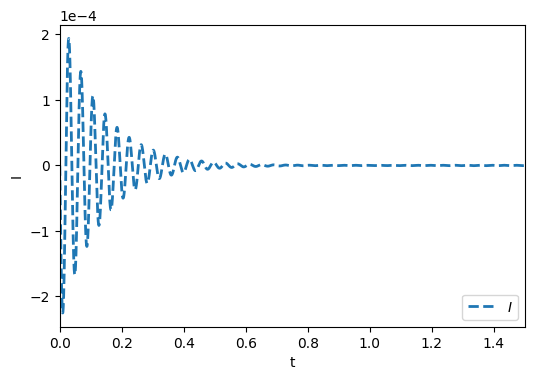
\includegraphics[width=.42\textwidth]{Fotos/SINen4.png}
        \end{figure}
        
        $R = 40\ \Omega ,\ \ U_{r} = 1.906\cdot10^{-8}\ J$):
        
        \begin{figure}[h]
            \centering
            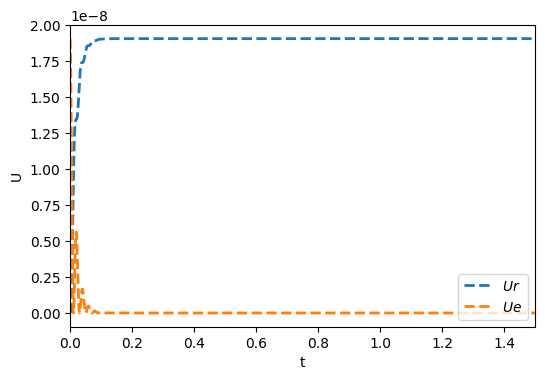
\includegraphics[width=.42\textwidth]{Fotos/SINen5.png}
            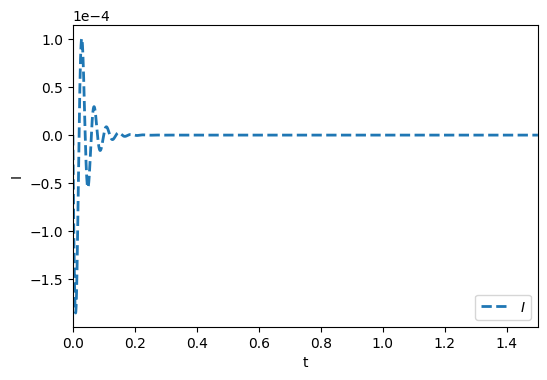
\includegraphics[width=.42\textwidth]{Fotos/SINen6.png}
        \end{figure}
        
        $R = 4000\ \Omega ,\ \ U_{r} = 1.892\cdot10^{-8}\ J$):
        
        \begin{figure}[h]
            \centering
            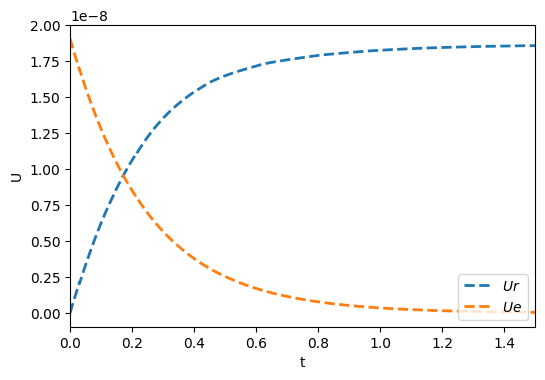
\includegraphics[width=.42\textwidth]{Fotos/SINen1.png}
            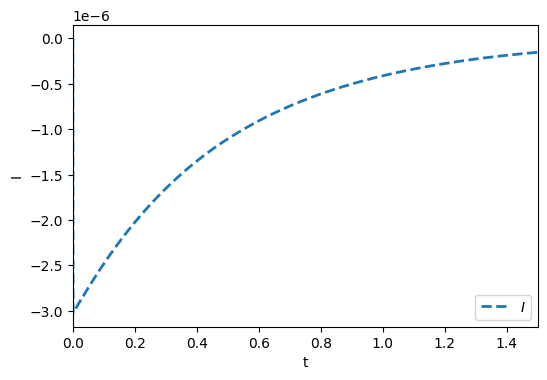
\includegraphics[width=.42\textwidth]{Fotos/SINen2.png}
        \end{figure}

\clearpage

\section{Circuito RLC en serie con generador}
    Cuando conectamos una fuente de voltaje a un circuito RLC, se proporciona energía para compensar para compensar la disipación de energía en la resistencia, de modo que la oscilación no atenúa.\\
    
    Estudiaremos ahora el caso de un generador de voltaje alterno conectado en serie con un condensador (inicialmente descargado), una resistencia y una bobina como indica la figura. 
    
    \begin{figure}[h]
        \centering
        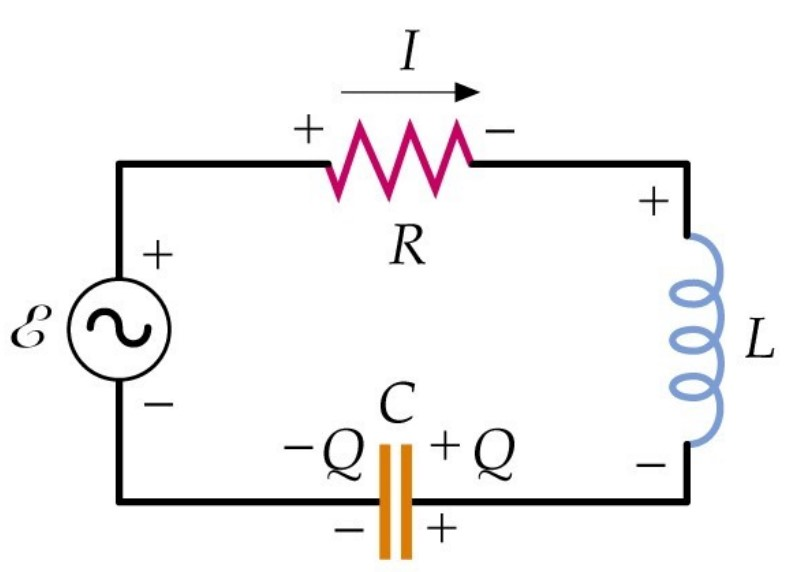
\includegraphics[width=.35\textwidth]{Fotos/RLCcon.jpg}
    \end{figure}
    
    El generador produce un voltaje alterno del tipo $V_{\varepsilon}(t)=V_0 cos(wt)$
    
    Aplicando la regla de Kirchhoff a la malla se obtiene:
    
    \[V_{\varepsilon}(t)-V_R(t)-V_L(t)-V_C(t)=V_{\varepsilon}(t)-IR-L \frac{dI}{dt}-\frac{Q}{C}=0\]
    
    que reordenando los términos conduce a la siguiente ecuación diferencial:
    
    \[L \frac{dI}{dt}+ IR+ \frac{Q}{C}= V_0 cos(wt)\]
    
    Suponiendo que el condensador está inicialmente descargado la ecuación anterior para la carga del condensador se puede reescribir como:
    
    \[L \frac{d^2Q}{dt^2}+R \frac{dQ}{dt}+ \frac{Q}{C}= V_0 cos(wt)\]
    
    El sistema tendrá un estado transitorio que ignoraremos, y al cabo de un tiempo llegará a un estado estacionario en el que oscilará con la frecuencia $w$ del generador. Ahora la ecuación diferencial que controla el sistema es equivalente a la de un oscilador armónico amortiguado y forzado. Una posible solución a la ecuación es:
    
    Para la carga, su amplitud y fase:
    
    \[Q(t)=Q_0 \cos{(\omega t - \delta)}\]
    
    \[Q_0= \frac{V_0/L}{\sqrt{(R\omega/L)^2+(\omega^2-1/LC)^2}} =\frac{V_0}{\omega \sqrt{R^2+(\omega L-1/\omega C)^2 }}=\frac{V_0}{\omega \sqrt{R^2+(X_L-X_C)^2}}\]
    
    \[\tan{\delta}=\frac{1}{R}(\omega L- \frac{1}{\omega C})=\frac{X_L-X_C}{R}\]\\
    
    Para la correspondiente corriente y su amplitud:
    
    \[I(t)=- \frac{dQ}{dt}= Q_0 \omega · \sin{(\omega t - \delta)}\]

    \[I_0= Q_0 \omega = \frac{V_0}{\sqrt{R^2+(X_L-X_C)^2}}= \frac{V_0}{Z}\]
    
    \hfill
    \subsection{Oscilador amortiguado y forzado}
    Una vez calculados los valores teóricos de $I$ y $\delta$ con el método de los fasores, usaremos el siguiente script con los valores de $R$, $C$, $L$, $V_{ef}$ y $f$ generados. Graficaremos el voltaje aplicado y la corriente en el circuito en función del tiempo. \\

    Para este apartado, el caso de un oscilador amortiguado y forzado, Graficaremos el voltaje aplicado y la corriente en el circuito respecto al tiempo. \\
    
    En segundo lugar, mediante el uso de los fasores, calcularemos la reactancia inductiva y capacitiva, la impedancia, el desfase y la intensidad pico y eficaz. Tal como muestra la figura:
    
    \begin{figure}[h]
        \centering
        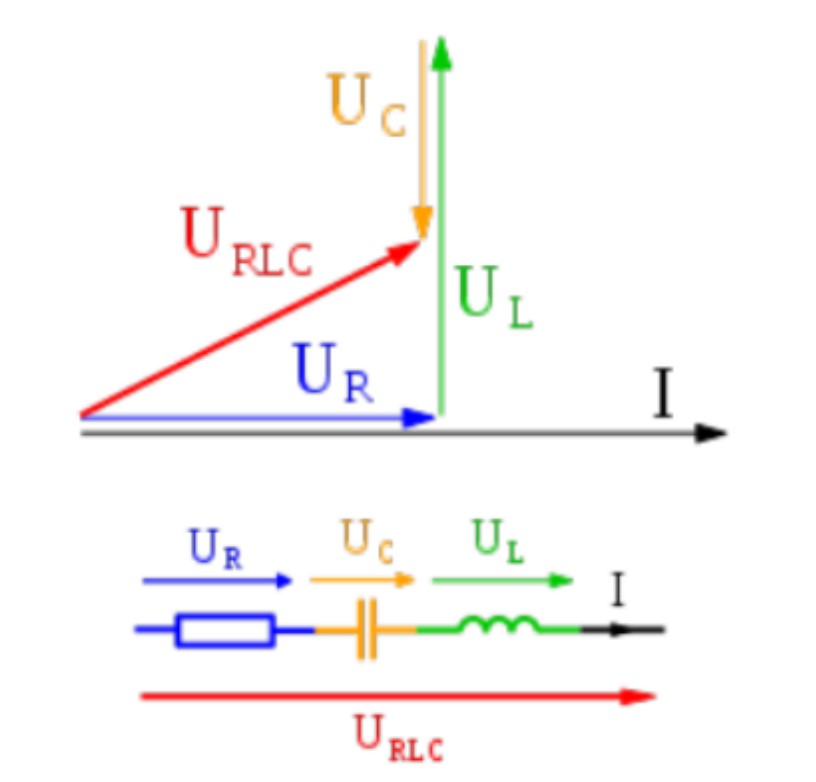
\includegraphics[width=.25\textwidth]{Fotos/fasores.jpg}
    \end{figure}
    
    Una vez calculados los valores teóricos de $I$ y $\delta$ con el método de los fasores, usaremos el siguiente script con los valores de $R$, $C$, $L$, $V_{ef}$ y $f$ generados. Recordar que los  valores eficaces se relacionan con los valores máximos según $V_{ef}=\frac{V_0}{\sqrt{2}}$.
    \begin{figure}[h]
        \centering
        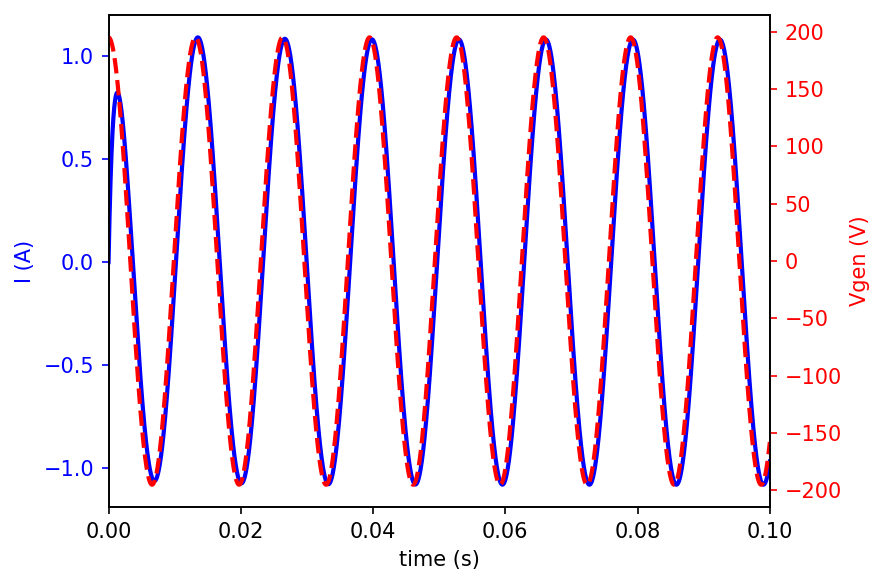
\includegraphics[width=.49\textwidth]{Fotos/CONfreq1.png}
        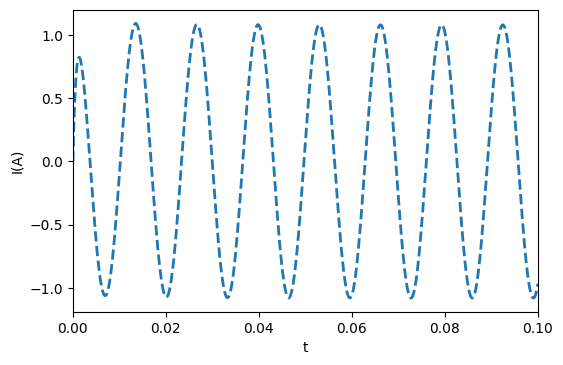
\includegraphics[width=.49\textwidth]{Fotos/CONfreq2.png}
    \end{figure}
    \begin{figure}[h]
        \centering
        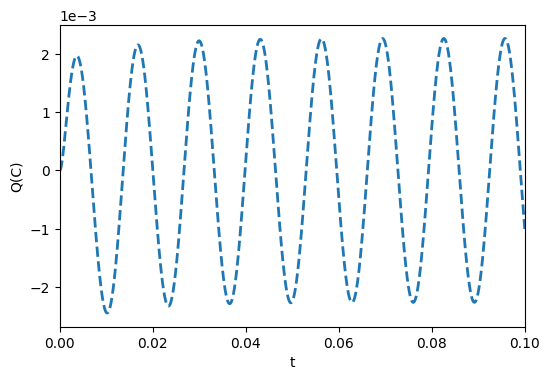
\includegraphics[width=.49\textwidth]{Fotos/CONfreq3.png}
        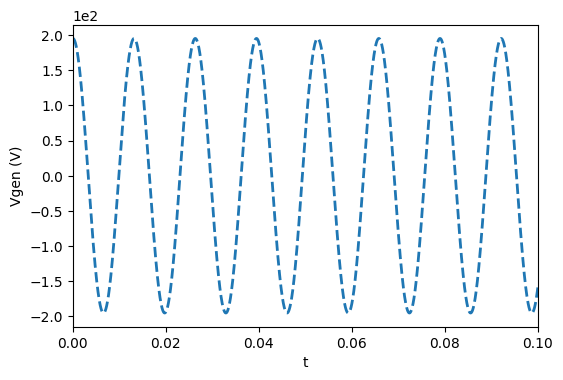
\includegraphics[width=.49\textwidth]{Fotos/CONfreq4.png}
    \end{figure}

\clearpage
    
    Por el método de los fasores obtenemos los siguientes datos:\\
    
    Imax $= 1.081\ A$\\
    Ieficaz $= 0.7644\ A$\\
    Periodo de I(t) $= 0.01316\ s$\\
    Frecuencia de I(t) $= 76\ Hz$\\
    Desfase $= 0.0266\ rad = 1.524^{\circ}$\\
    
    Destacar que existe un pequeño desfase entre el voltaje y la intensidad, que podemos observar en la pequeña distancia entre la curva azul y la roja de la figura. Podemos afirmar que el desfase entre ambas es muy pequeño y por tanto ambas magnitudes se comporten de manera muy parecida.\\
    
    \vspace{1.5cm}
    \subsection{Estudio de la resonancia}
    Con los valores introducidos anteriormente (modificando la resistencia a pocos $\Omega$) realizamos la gráfica de $I$ en función de la frecuencia. Destacar que el máximo de $I$ se obtiene para la frecuencia de resonancia $f_{res} = \frac{1}{2\pi \sqrt{LC}}$.\\
    
    Obtenemos valores para la frecuencia de resonancia analíticamente y numéricamente y observamos que coinciden en $f_{res} = 52.36\ Hz$
    
    \begin{figure}[h]
        \centering
        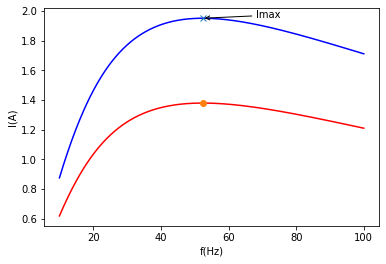
\includegraphics[width=.49\textwidth]{Fotos/CONreso.png}
    \end{figure}
        
    En la figura graficamos la intensidad frente a la frecuencia, siendo la curva azul la intensidad máxima (que se obtiene para la frecuencia de resonancia) y la curva roja la intensidad efectiva.
    

\clearpage
\section{Códigos}
    \noindent Adjunto en este apartado los códigos en python utilizados para la realización de esta práctica. Recordar que los siguientes enlaces están restringidos a lectores con correos electrónicos asociados a la Universidad de Alicante: \\
    
    \noindent Circuito RLC en serie sin generador: \href{https://colab.research.google.com/drive/13GIrx54IEKJPyuWR2zWD0QK0Csr4QSl8?usp=sharing}{Código sin generador} 
    
    \vspace{.3cm}
    \noindent Circuito RLC en serie con generador: \href{https://colab.research.google.com/drive/1wUlrRMlpS3oeaVdSZSz8MbYVYWOmFezm?usp=sharing}{Código con generador} 

\end{document}